
\chapter{Projekt oraz implementacja rozwiązania}

\section{Wstęp}
W ramach pracy inżynierskiej opracowano kompleksowe narzędzie \textbf{gptester}, które wykorzystuje zaawansowane modele językowe do analizy statycznej kodu.
Narzędzie to wykorzystuje domyślnie model GPT-4 do generowania raportów na temat jakości kodu oraz proponowania napraw, ze szczególnym uwzględnieniem bezpieczeństwa kodu.

\section{Architektura systemu}
\subsection{Ogólny opis}
\textbf{GPTester} jest programem napisanym w języku Python, wykorzystującym model GPT-4 (lub GPT-3.5-turbo) dostarczony przez OpenAI.
Jest zaprojektowany do uruchamiania z linii poleceń, a wyniki jego pracy są zapisywane w pliku formatu markdown oraz do osobnego katalogu z plikami wynikowymi zawierającymi poprawiony kod.
Praktyczną funkcjonalność zapewnia wykorzystanie metod git, takich jak tworzenie i zapisywanie łatek (ang. patch), co umożliwia wygodne wprowadzanie poprawek do kodu oraz kontrolę wersji i łatwe scalanie kodu.

\subsection{Schemat blokowy}
\label{subsec:schemat_blokowy}

\begin{landscape}
\begin{figure}[p]
    \centering
    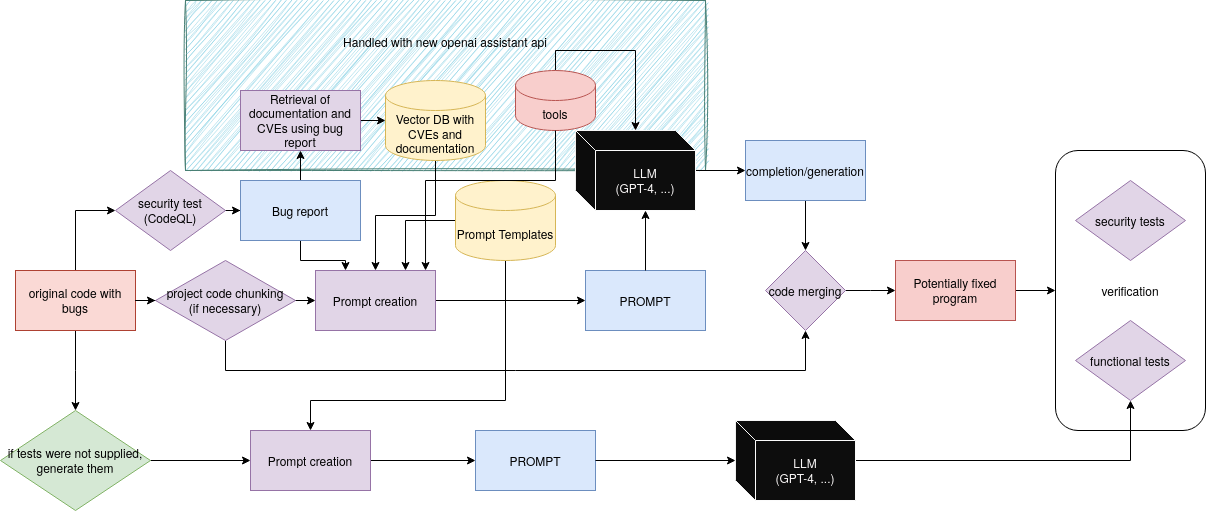
\includegraphics[width=\linewidth]{img/gptester.drawio.png}
    \caption{Schemat blokowy działania aplikacji \textit{gptester}}
    \label{fig:schemat_blokowy}
\end{figure}
\end{landscape}

\subsubsection{Dane wejściowe i wstępne przetwarzanie}
\begin{figure}[h]
    \centering
    % Adjust the clip and trim parameters as needed: {left bottom right top}
    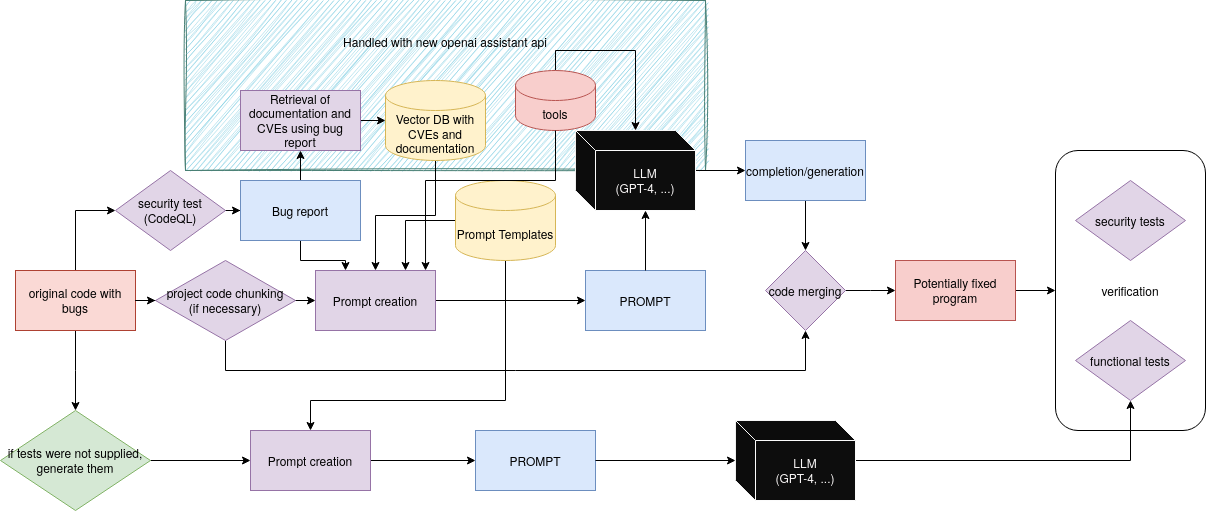
\includegraphics[clip, trim=0cm 4cm 29cm 6cm, width=0.9\linewidth]{img/gptester.drawio.png}
    \caption{dane wejściowe w schemacie blokowym}
    \label{fig:przyciety_obrazek}
\end{figure}
Proces rozpoczyna się od dostarczenia \texttt{oryginalnego kodu z błędami}. Następnie jeśli użytkownik przygotował środowisko dla CodeQL zostanie ono wykorzystane do wstępnej analizy, a dane wynikowe zostaną wykorzystane do wzbogacenia poleceń(promptów). 
W przeciwnym wypadku polecenie(prompt) zostanie skreowany na podstawie danych posiadanych. 

\subsubsection{Generacja testów funkcjonalnych}
\begin{figure}[h]
    \centering
    % Adjust the clip and trim parameters as needed: {left bottom right top}
    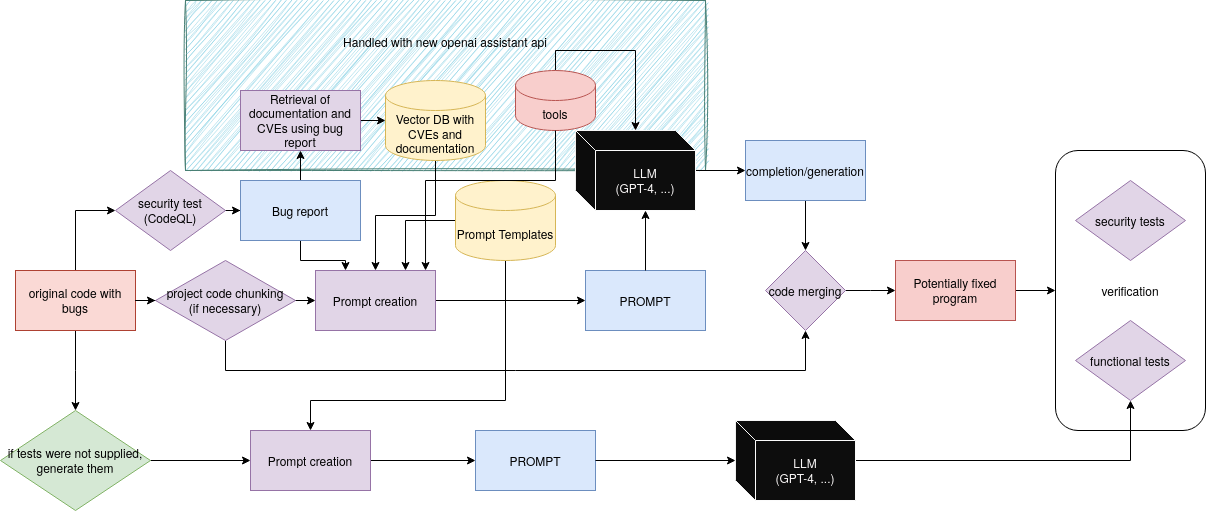
\includegraphics[clip, trim=0cm 0cm 0cm 13cm, width=0.9\linewidth]{img/gptester.drawio.png}
    \caption{Część schematu opisująca proces generatora testów funkcjonalnych}
    \label{fig:przyciety_obrazz}
\end{figure}

Jeżeli testy funkcjonalne dla naszego kodu nie zostały zapewnione, zostaną one wygenerowane za pomocą osobnego agenta. 
Jest to funkcja nadal testowana, która w przyszłości ma za zadanie generować testy funkcjonalne dla kodu, który ich nie posiada. 
Problemem jest duża ilość kodu dla średnich i dużych projektów, dlatego zalecane jest dostarczenie własnego modułu testów funkcjonalnych.

\subsection{Wzbogacanie zapytań\footnote{ang. prompt}}
\begin{figure}[h]
    \centering
    % Adjust the clip and trim parameters as needed: {left bottom right top}
    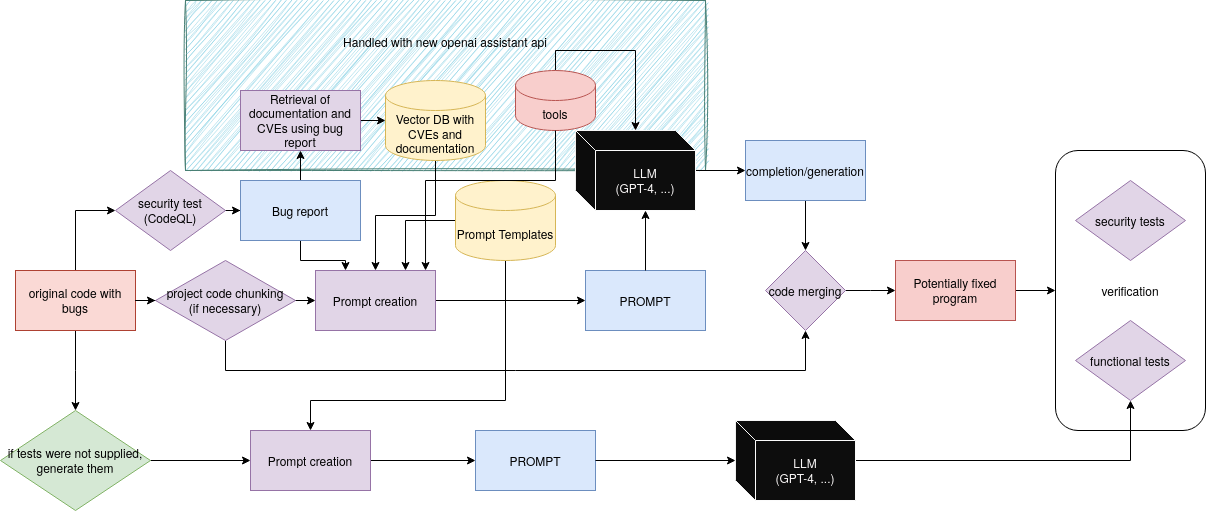
\includegraphics[clip, trim=3cm 11cm 3cm 0cm, width=0.9\linewidth]{img/gptester.drawio.png}
    \caption{Część schematu opisująca proces RAG}
    \label{fig:RAG-schemat}
\end{figure}

Dla uzyskania jak najlepszych wyników oraz zapewnienia najnowszej dostępnej wiedzy na temat podatności wykorzystywane zostaje RAG, aby wzbogacić monit o dodatkowe informacje. Są to informacje otrzymane z CodeQL, które zostają użyte do semantycznego wyszukania powiązanych wpisów w bazie danych CVE. 
Jeżeli CodeQL nie został użyty, monit zostaje wzbogacony o informacje z bazy CVE, które zostały wyszukane semantycznie w wektorowej bazie wiedzy. W tej chwili o użyciu danych z bazy wiedzy decyduje wybrany model OpenAI, dzięki nowym możliwością API. 
Nowe możliwości API jak własne narzędzia dla LLM, code interpreter (interpreter kodu) oraz semantic search (semantyczne wyszukiwanie) zostały wprowadzone 06.11.2023r.
Sprawia to, że niniejszy własny kod do wzbogacania monitów jest niepotrzebny, ale w przyszłości może zostać użyty do wzbogacania monitów o dodatkowe informacje dla modeli otwartoźródłowych. 
\begin{listing}
    \begin{minted}{python}  
def get_embedding(text, model="text-embedding-ada-002"): # alternatively use code-embedding-ada
    text = str(text)
    text = text.replace("\n", " ")
    if len(text) != 0:
        return openai.Embedding.create(input=[text], model=model)["data"][0]["embedding"]
    return [0.0] * 1536

    \end{minted}
    \caption{Kod tworzący reprezentację wektorową tekstu za pomocą API OpenAI, domyślnie `text-embedding-ada-002', (models.py)} 
    \label{listing:vector_embedding}
\end{listing}
    
\begin{listing}
    \begin{minted}{python}  
    def relevance_for(self, query: str) -> float:
        embedding = get_embedding(query)
        task = get_embedding(self.name)
        score = cosine(task, embedding)
        return score
    \end{minted}
    \caption{Kod porównujący semantyczną odległość (models.py)} 
    \label{listing:vector_relevance}
\end{listing}
    
Przedstawione zostały rzeczywiste skrawki kodu znajdujące się w projekcie, natomiast w testach oraz podczas działania na modelach komeryjnych OpenAI używane są funkcje dostępne za pomocą API.

\definecolor{light-blue}{rgb}{0.8,0.85,1}

\subsubsection{Tworzenie monitów i interakcja z LLM}
\begin{figure}[h]
    \centering
    % Adjust the clip and trim parameters as needed: {left bottom right top}
    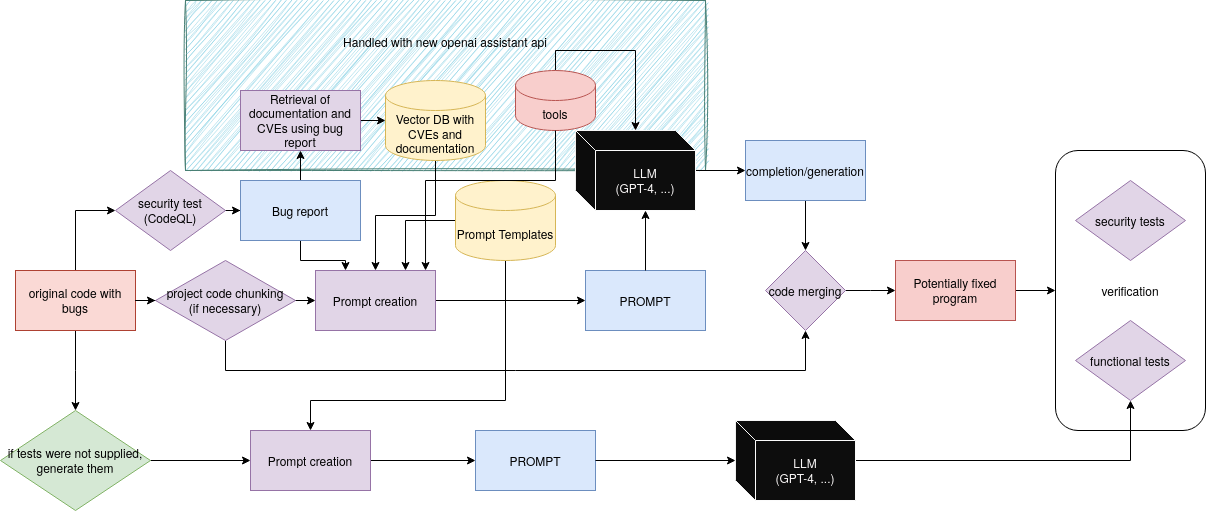
\includegraphics[clip, trim=3cm 10cm 3cm 0cm, width=0.9\linewidth]{img/gptester.drawio.png}
    \caption{Część schematu opisująca proces RAG}
    \label{fig:przyciety_obraz}
\end{figure}
Dla każdej części kodu badanego projektu opdowiednio mieszczącej się w oknie kontekstu dla modeli, tworzony jest \textbf{PROMPT} (monit), który jest następnie przetwarzany przez `\textbf{LLM (GPT-4, \ldots)}`. 
W tym celu wykorzywane są \textbf{Prompt templates} (szablony monitów) oraz semantycznie wyszukane skrawki z \textbf{Vector DB with CVEs and documentation} (wektorowa baza danych z CVE oraz dokumentacją).

Tak spreparowane zapytanie jest następnie zadane modelowi językowemu, który identyfikuje podatności oraz proponuje poprawki.

\subsubsection{Generowanie kodu i scalanie}
\begin{figure}[h]
    \centering
    % Adjust the clip and trim parameters as needed: {left bottom right top}
    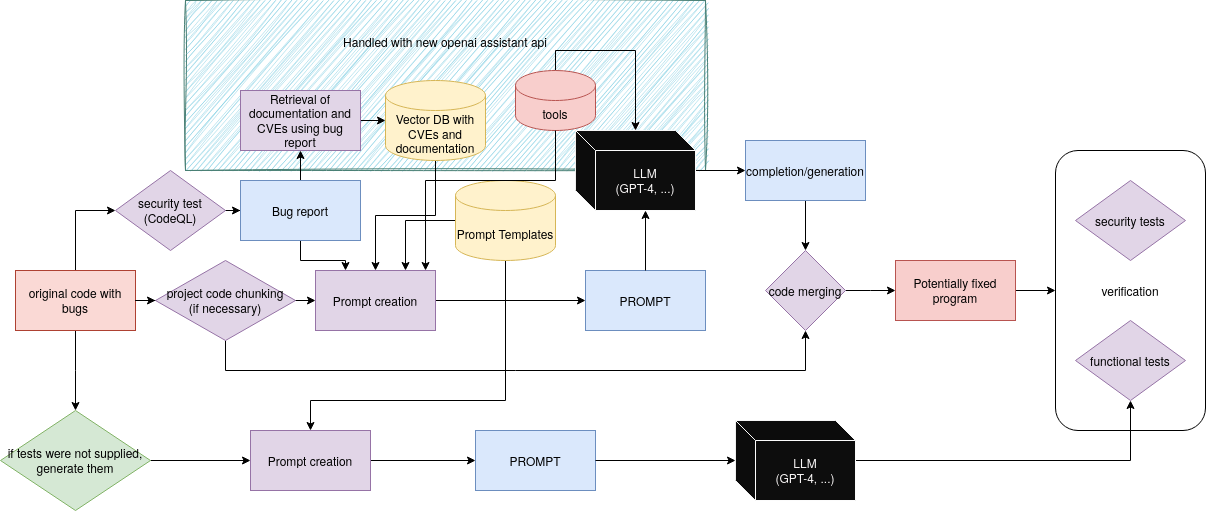
\includegraphics[clip, trim=12cm 6cm 6cm 0cm, width=0.9\linewidth]{img/gptester.drawio.png}
    \caption{Czarna skrzynka - LLM (Large Language Model)}
    \label{fig:przyciety_obraz-generowanie}
\end{figure}
LLM generuje \texttt{uzupełnienie/generacje kodu} oraz raport, które są następnie łączone \textbf{(code merging)} w potencjalnie \texttt{naprawiony program}. Proces ten wykorzystuje również \textbf{narzędzia}
(code interpreter, knowledge retrieval, file writing, running tests, \dots), aby ułatwić obróbkę wyników oraz wzbogacić generację.

\subsubsection{Testy i weryfikacja}
\begin{figure}[h]
    \centering
    % Adjust the clip and trim parameters as needed: {left bottom right top}
    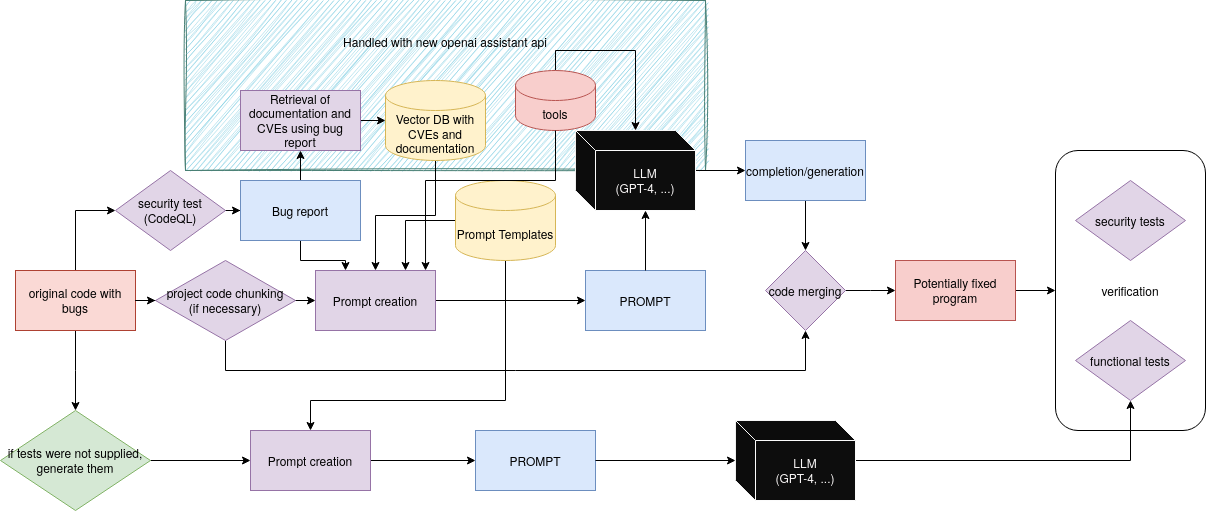
\includegraphics[clip, trim=25cm 2cm 0cm 4cm, width=0.9\linewidth]{img/gptester.drawio.png}
    \caption{Czarna skrzynka - LLM (Large Language Model)}
    \label{fig:przyciety_obraz2}
\end{figure}
W ramach procesu weryfikacyjnego, naprawiony kod jest poddawany \textbf{testom bezpieczeństwa} oraz \textbf{testom funkcjonalnym}, mając na celu zapewnienie, że wprowadzone poprawki nie generują nowych defektów oraz że aplikacja funkcjonuje zgodnie z założeniami. W literaturze źródłowej, na której opiera się niniejsza praca inżynierska, do realizacji testów bezpieczeństwa stosowane są narzędzia takie jak CodeQL, czy ASAN/UBSAN, które umożliwiają wykrycie podatności w kodzie. Proces ten jest zautomatyzowany, co jest kluczowe dla przeprowadzenia badań w skali naukowej. Jednakże, z powodu specyfiki integracji CodeQL w ramach realizowanego projektu, jego wykorzystanie do testów nie jest rekomendowane, gdyż nie zapewnia wiarygodności wyników. W związku z tym, testy bezpieczeństwa są przeprowadzane manualnie w celu potwierdzenia prawidłowości działania systemu, podczas gdy testy funkcjonalne realizowane są w sposób automatyczny. 
Zaleca się wskazanie dedykowanego modułu testowego dla skanowanego projektu.
\subsubsection{Dokumentacja i raportowanie}
Wyniki pracy \textbf{gptester} są dokumentowane w raporcie o błędach, po czym raport jest zapisywany w plikach markdown, a poprawione pliki z kodem w katalogu `fixed` z odpowiednim znacznikiem czasowym. W przyszłości poprawki będą wprowadzane do bazy kodu za pomocą git patch.

\subsubsection{Podsumowanie}
Diagram blokowy przedstawia kompleksowy proces analizy i naprawy kodu, który jest silnie zależny od danych wejściowych (kod źródłowy i testy bezpieczeństwa), zaawansowanych algorytmów przetwarzania (duże modele językowe) oraz dokładności w generowaniu poprawek kodu i ich weryfikacji. Cały proces jest automatyzowany, a weryfikacja jest możliwa na otrzymanych wynikach.


\section{Implementacja oraz użycie}
\subsection{Środowisko programistyczne i wymagania}

Projekt \textbf{gptester} został opracowany w środowisku programistycznym Python, z wykorzystaniem modelu GPT-4 dostarczonego przez OpenAI. Proces konfiguracji środowiska rozpoczyna się od przygotowania odpowiedniego środowiska Pythona i zainstalowania niezbędnych zależności.

Wymagania wstępne:
\begin{itemize}
    \item Python w wersji >3.7 – Język programowania wykorzystany do napisania `gptester`.
    \item Dostęp do internetu – Niezbędny do pobrania zależności i interakcji z modelem GPT-4 przez API OpenAI.
\end{itemize}

Instalacja zależności:
\begin{listing}
    \begin{minted}{bash}
pip install -r requirements.txt
\end{minted}
\end{listing}

Plik `requirements.txt` zawiera wszystkie niezbędne biblioteki Pythona wymagane do działania \textbf{gptester}. 
Instalacja zależności jest prosta i może być wykonana w terminalu lub wirtualnym środowisku Pythona, co jest zalecane w celu uniknięcia konfliktów z istniejącymi pakietami.

Do poprawnego działania wspieranego CodeQL należy zainstalować narzędzie CodeQL - CLI, które jest dostępne na stronie \url{https://codeql.github.com/}
\subsection{Uruchomienie programu}

\begin{listing}
    \begin{minted}{bash}
        cd gptester
        python main.py -h
    \end{minted}
\end{listing}
lub 
\begin{listing}
    \begin{minted}{bash}
        cd gptester
        chmod +x main.py
        ./main.py --help
    \end{minted}
\end{listing}

\subsection{Funkcje programu}

Program \textbf{gptester} został zaprojektowany jako wszechstronne narzędzie do analizy statycznej kodu, korzystając z zaawansowanych modeli językowych do wykrywania i naprawiania błędów bezpieczeństwa w kodzie. Wersja \texttt{assistant-0.5.2-beta} programu oferuje szereg funkcji, które są dostępne za pomocą argumentów linii poleceń, umożliwiając szeroką konfigurację i dostosowanie do specyficznych potrzeb analizy.

\begin{itemize}
    \item \textbf{-h, --help}: Wyświetla pomoc programu, prezentując dostępne opcje i ich krótki opis, co ułatwia szybkie zrozumienie możliwości programu.
    \item \textbf{-v, --verbose}: Aktywuje tryb szczegółowych informacji, dzięki czemu \texttt{gptester} prezentuje dodatkowe informacje o każdym etapie przetwarzania, co jest przydatne do debugowania i głębszej analizy działania.
    \item \textbf{-f, --format}: Określa format pliku wyjściowego rezultatu, dla najnowszej wersji programu domyślnie jest to csv, ale może zostać zmieniony na markdown, jak domyślnie w starszych wersjach.
    \item \textbf{-m MODEL, --model MODEL}: Umożliwia wybór modelu językowego do analizy kodu, z domyślnym ustawieniem na "gpt-4-1106-preview". Pozwala na dostosowanie narzędzia do specyficznych wymagań projektu poprzez wybór innego dostępnego modelu.
    \item \textbf{-r, --retrieval}: Włącza Generację Wspomaganą Odnajdywaniem (Retrieval Augmented Generation - RAG) dla analizy kodu, zwiększając precyzję identyfikacji podatności przez odwołanie się do zewnętrznych baz wiedzy.
    \item \textbf{-k FILE\_TO\_KNOW, --file-to-know FILE\_TO\_KNOW}: Pozwala na wskazanie pliku, który ma być załączony do bazy wiedzy, co może pomóc w poprawie kontekstu analizy. Domyślnie ustawione na bazę danych CVE w formacie CSV.
    \item \textbf{-i IGNORE, --ignore IGNORE}: Umożliwia podanie ścieżki do pliku .gitignore, aby zignorować określone pliki podczas skanowania, co pomaga skupić się na kluczowych elementach kodu.
    \item \textbf{-p PATCH\_FILE, --patch-file PATCH\_FILE}: Określa ścieżkę dla wygenerowanego pliku z poprawkami, umożliwiając łatwe śledzenie i aplikowanie sugerowanych zmian w kodzie.
    \item \textbf{-o OUTPUT, --output OUTPUT}: Określa ścieżkę i nazwę pliku, do którego zostaną zapisane wyniki analizy. Pozwala na elastyczne zarządzanie dokumentacją wyników.
    \item \textbf{-t TESTS, --tests TESTS}: Wskazuje ścieżkę do testów funkcjonalnych, które mają być wykonane na projekcie. Ułatwia integrację z istniejącymi procedurami testowymi i pozwala na automatyczne generowanie testów, jeśli nie zostaną dostarczone.
    \item \textbf{-c, --codeql}: Włącza integrację z CodeQL, zaawansowanym narzędziem do analizy kodu. Wymaga zainstalowania narzędzia CodeQL-CLI i jest przeznaczone do wykrywania bardziej złożonych podatności.
    \item \textbf{--command COMMAND}: Umożliwia określenie polecenia budowania projektu, co jest niezbędne do prawidłowej integracji z CodeQL, szczególnie gdy w projekcie nie ma pliku cmake lub podobnego. Domyślnie ustawione na "make".
    \item \textbf{--language LANGUAGE}: Pozwala na określenie języka programowania projektu dla analizy CodeQL, z domyślnym ustawieniem na "cpp". Umożliwia dostosowanie analizy do różnych środowisk programistycznych.
\end{itemize}
\begin{figure}[H]
    \centering
    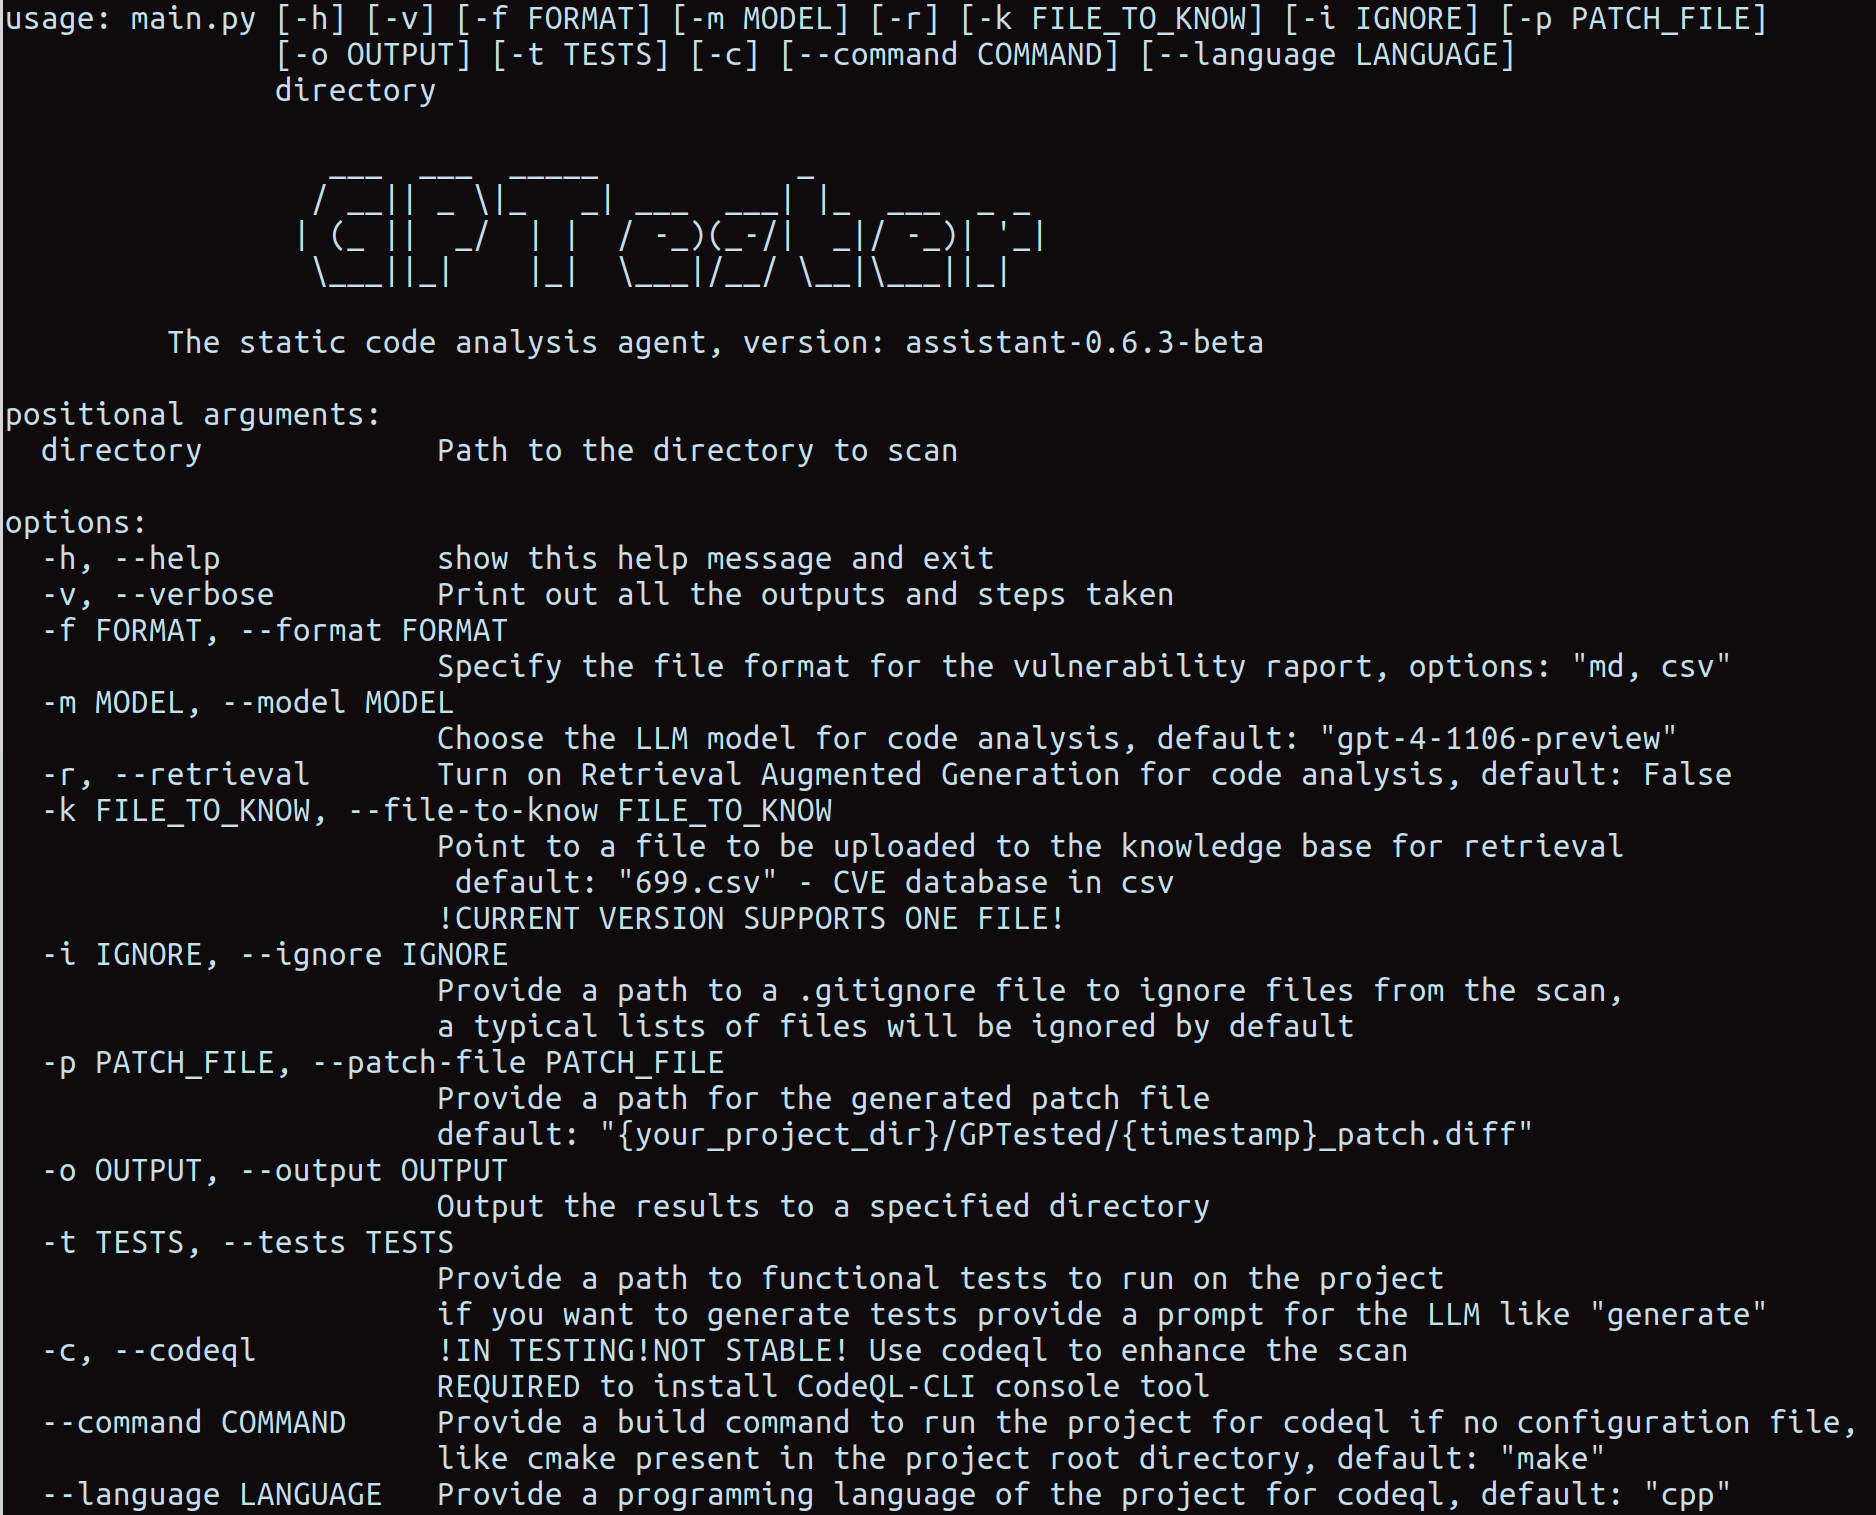
\includegraphics[width=\linewidth]{img/gptester-help.png}
    \caption{Wiadomość pomocnicza aplikacji \textit{gptester}}
    \label{fig:gptester-help}
\end{figure}

Przykład użycia z pełną konfiguracją:

\begin{listing}
    \begin{minted}{bash}
./main.py /ścieżka/do/projektu --verbose --format csv --model "gpt-4-1106-preview" --output "moj_raport.md" --tests "/ścieżka/do/testów" --codeql --command "mvn -B -DskipTests -DskipAssembly" --language "java"
\end{minted}
\end{listing}

W powyższym przykładzie, gptester analizuje kod znajdujący się w podanej ścieżce, z włączonym trybem szczegółowych informacji, korzystając z modelu GPT-4, zapisując wyniki do określonego pliku raportu, wykonując testy funkcjonalne, integrując z CodeQL, używając polecenia \texttt{mvn -B -DskipTests -DskipAssembly} do budowy projektu w języku Java. Budowa projektu jest wymagana przez CodeQL, dlatego ten argument jest wykorzystywany jedynie przy integracji z CodeQL. CdodeQL musi być zainstalowany i skonfigurowany w środowisku, aby analiza mogła się powieść, a podana komenda powinna budować projekt w trybie czystym\footnote{ang. clean build}, aby przez kompilator niewykorzystywane były artefakty z poprzednich budowań.

\section{Integracja z CodeQL}
\label{sec:integracja_codeql}

Integracja GPTester z CodeQL znacznie rozszerza jego funkcjonalność analizy statycznej kodu. CodeQL, opracowany przez Microsoft, a dokładnie GitHub, to zaawansowane narzędzie do semantycznej analizy kodu, które umożliwia wykrywanie złożonych podatności i błędów bezpieczeństwa.

\textbf{Główne cechy integracji z CodeQL:}
\begin{itemize}
    \item \textbf{Zaawansowana Analiza Bezpieczeństwa}: CodeQL przekształca kod źródłowy w zapytywalną formę, co pozwala na przeprowadzenie głębokich analiz w poszukiwaniu subtelnych luk bezpieczeństwa.
    \item \textbf{Wsparcie Dla Wielu Języków}: Obsługa różnych języków programowania przez CodeQL, takich jak C++, Java, Python, co jest wykorzystywane przez `gptester` do analizy różnorodnych projektów.
    \item \textbf{Konfiguracja Procesu Budowania}: Możliwość dostosowania polecenia budowania projektu za pomocą opcji \texttt{--command}, niezbędna w przypadku braku pliku konfiguracyjnego jak cmake w katalogu głównym.
    \item \textbf{Elastyczność Analizy}: Użytkownik może wybrać między szybkimi analizami a bardziej dogłębnymi badaniami, co umożliwia dostosowanie procesu do konkretnych wymagań projektu.
    \item \textbf{Automatyzacja Wykrywania Podatności}: CodeQL automatyzuje proces wykrywania podatności, zwiększając skuteczność i efektywność analizy bezpieczeństwa kodu.
\end{itemize}

Integracja z CodeQL czyni \textbf{gptester} narzędziem nie tylko do wykrywania błędów syntaktycznych i strukturalnych, ale także do efektywnego identyfikowania subtelniejszych problemów bezpieczeństwa, które mogą umknąć podczas standardowych analiz.
Do działania CodeQL niezbędne jest zainstalowanie CodeQL CLI, które można pobrać ze strony GitHub.

\section{Modele językowe}
\label{sec:modele_jezykowe}

W ramach projektu \textbf{gptester} zaimplementowano zaawansowane modele językowe dostarczone przez OpenAI, w szczególności GPT-4, które odegrały kluczową rolę w procesie analizy statycznej kodu. Modele te wykorzystują techniki uczenia maszynowego i sztucznej inteligencji do generowania odpowiedzi na podstawie dostarczonych danych.

\subsection{Wykorzystanie Modeli Językowych}
Modele językowe w projekcie \textbf{gptester} są wykorzystywane do identyfikacji i sugerowania potencjalnych napraw błędów w kodzie źródłowym. Proces ten opiera się na zaawansowanej analizie kontekstu i semantyki kodu, co pozwala na precyzyjne wykrywanie nawet subtelnych podatności.

\subsection{Dostępne Modele}
Projekt integruje różne wersje modeli GPT, z dominującą rolą GPT-4, który charakteryzuje się wyższą zdolnością do zrozumienia złożonych zapytań i generowania bardziej precyzyjnych odpowiedzi. Dostępność innych modeli, takich jak GPT-3.5, zapewnia elastyczność w doborze narzędzia w zależności od specyficznych wymagań analizy. 

\subsubsection{Modele otwartoźródłowe}
W przyszłości wdrożone zostaną także modele otwartoźródłowe, za pomocą narzędzia Ollama. Dostępne będą między innymi: Llama2, GPT-J, Mistral, Falcon, czy jakikolwiek model dostępny w repozytoriach Ollama. Narzędzie to pozwala na łatwe pobieranie modeli, konteneryzowane uruchamianie, a także dostęp za pomocą API. Zapewni to jeszcze większą elastyczność i dostosowanie do potrzeb projektu.

\subsection{Inżynieria Poleceń (Promptów)}
Kluczowym aspektem wykorzystania modeli językowych jest inżynieria promptów, czyli proces projektowania i optymalizowania zapytań w celu uzyskania jak najbardziej trafnych odpowiedzi od modelu. W projekt \textbf{gptester} zaimplementowano zestaw specjalnie opracowanych promptów, które są dostosowane do identyfikacji różnych rodzajów błędów i podatności w kodzie.

Polecenie systemowe używane dla agenta odpowiedzialnego za identyfikację i naprawę błędów, zapisującego wyniki w formacie csv wygląda następująco:

\begin{framed}
\scriptsize
\begin{verbatim}
You are a top-tier security specialist. You have been tasked with finding vulnerabilities and 
security bugs in a program. You will be given either a code snippet, a whole codefile or 
multiple files and optionally a description of errors found by CodeQL. 

You must find all the security vulnerabilities, list them and append all of them to the file 
"GPTest.csv" in the following format:
Vulnerability Name; File Name; Line Number; Severity(impact/risk); Description; Solution;

Next you will write the fixed code to a file with the same name as the original file in 
a new folder called "fixed". Always write the whole file with complete functional code. 
Always write the new file without asking for confirmation or more context, even when you 
only have a snippet of code write it to a new file.

write_file = {
    "name": "write_file",
    "description": "Writes content to a specified file.",
    "parameters": {
        "type": "object",
        "properties": {
            "filename": {"type": "string"},
            "content": {"type": "string"}
        },
        "required": ["filename", "content"]
    }
}

append_to_csv = {
    "name": "append_to_csv",
    "description": "Appends a row to an existing CSV file using a semicolon as the delimiter.",
    "parameters": {
        "type": "object",
        "properties": {
            "file_path": {
                "type": "string",
                "description": "The path to the CSV file to which the row will be appended."
            },
            "row_data": {
                "type": "array",
                "description": "A list of values to be formatted into a CSV row and appended 
                                to the file.",
                "items": {
                    "type": "string"
                }
            }
        },
        "required": ["file_path", "row_data"]
    }
}
\end{verbatim}
\end{framed}
\normalsize


Można zauważyć, że prompty są złożone z dwóch części: pierwsza część to opis zadania, które ma wykonać model, a druga część to opis funkcji, która ma zostać użyta do zapisania plików. W ten sposób model jest w stanie zrozumieć kontekst zadania oraz wykonać odpowiednie operacje. Użycie funkcji oraz zwrócenie odpowiedzi przez tę funkcję jest zaimplementowane w ai/assistant.py oraz tools.py \ref{lst:api_openai}. Lokalizacja zapisywanych plików jest zmieniana przez kod i niezależna od modelu.

Prompt dla innych punktów końcowych API będzie wyglądał inaczej. Niezbędna jest wówczas implementacja parsera dla odpowiedzi od modelu językowego, aby wyodrębnić odpowiednie informacje i zapisać do plików.

\subsection{Integracja z API OpenAI}
\label{sec:integracja_openai}
Komunikacja z modelami językowymi odbywa się za pośrednictwem API OpenAI, co umożliwia wykorzystanie najnowszych osiągnięć w dziedzinie sztucznej inteligencji bez konieczności posiadania zasobów obliczeniowych do lokalnego trenowania modeli. 

Można wyróżnić trzy główne sposoby komunikacji z API OpenAI:
\begin{enumerate}
    \item \textbf{Completion(Komplecja/Uzupełnienie)}: Punkt końcowy API zakończenia otrzymał ostateczną aktualizację w lipcu 2023 r. i ma inny interfejs niż nowy punkt końcowy dopełnienia czatu\footnote{ang. Chat Completion}. Zamiast danych wejściowych będących listą komunikatów, danymi wejściowymi jest dowolny ciąg tekstowy zwany poleceniem\footnote{ang. prompt}.

    Przykładowe wywołanie starszego interfejsu API Completions wygląda następująco:
    \begin{listing}
        \begin{minted}{python}
from openai import OpenAI
client = OpenAI()

response = client.completions.create(
  model="gpt-3.5-turbo-instruct",
  prompt="Write a tagline for an ice cream shop."
)
        \end{minted}
    \end{listing}
    \item \textbf{ChatCompletion(Komplecja/Uzupełnienie dialogowe)}: Modele czatu przyjmują listę wiadomości jako dane wejściowe i zwracają wiadomość wygenerowaną przez model jako dane wyjściowe. Chociaż format czatu został zaprojektowany tak, aby ułatwić wieloturowe rozmowy, jest równie przydatny w przypadku zadań jednoturowych bez żadnej rozmowy.

    Przykładowe wywołanie interfejsu API Chat Completions wygląda następująco:
    \begin{listing}[H]
        \begin{minted}{python}
from openai import OpenAI
client = OpenAI()

response = client.chat.completions.create(
  model="gpt-3.5-turbo",
  messages=[
    {"role": "system", "content": "You are a helpful assistant."},
    {"role": "user", "content": "Who won the world series in 2020?"},
    {"role": "assistant", "content": "The Los Angeles Dodgers won the World Series in 2020."},
    {"role": "user", "content": "Where was it played?"}
  ]
)
            \end{minted}
        \end{listing}
        \item \textbf{Assistant(Asystent)}: Punkt końcowy API Asystentów pozwala na tworzenie asystentów AI w ramach własnych aplikacji. Asystent posiada instrukcje i może wykorzystywać modele, narzędzia oraz wiedzę do odpowiadania na zapytania użytkowników. API Asystentów obecnie obsługuje trzy typy narzędzi: Interpreter Kodu, Pobieranie oraz Wywoływanie Funkcji. W przyszłości planujemy udostępnić więcej narzędzi stworzonych przez OpenAI oraz umożliwić dostarczanie własnych narzędzi na naszej platformie.
        
        Przykładowe wywołanie interfejsu API Asystentów wygląda następująco:
        \begin{listing}
            \begin{minted}{python}
assistant = client.beta.assistants.create(
    name="Math Tutor",
    instructions="You are a personal math tutor. Write and run code to answer math questions.",
    tools=[{"type": "code_interpreter"}],
    model="gpt-4-1106-preview"
)
            \end{minted}
        \end{listing}
\end{enumerate}

\subsection{Implementacja w projekcie}
Kod użyty w projekcie został dostosowany do nowego interfejsu Assistant API, który jest zgodny z najnowszymi wersjami modeli językowych. W projekcie znajduje się także kod wykorzystujący starsze interfejsy API, który może być użyty w przypadku starszych wersji modeli językowych. Ten kod oraz własna implementacja bazy wektorowej wynika z daty wprowadzenia punktu końcowego API asystantów, który został wprowadzony 06.11.2023r.
Kod użyty w projekcie znajduje się w pliku `ai/assistant.py` i wygląda następująco\footnote{wersja programu: \texttt{assistant-0.2.2-beta}, w nowszej wersji znajduje się większa ilość kodu, który nie jest istotny dla niniejszej pracy, jak nadpisywanie lokalizacji plików}:
\newgeometry{top=0.5cm, left=2cm,right=2cm, bottom=3cm}

\begin{listing}
    \begin{minted}[fontsize=\scriptsize]{python}
class Assistant():
    def __init__(self, role: str, name: str = "Assistant", model: str = 'gpt-3.5-turbo-1106', iol: IOlog = None, tools = None, messages = None) -> None:
        self.name = name
        self.iol = iol
        self.instructions = role
        self.assistant = client.beta.assistants.create(
            name=name,
            instructions=self.instructions,
            model=model,
            tools=tools if tools else [{"type": "code_interpreter"}, {"type": "retrieval"}]
        )
        self.thread = client.beta.threads.create(messages = messages)
    # pominięte metody przekształcania wiadomości, pozwalające na łatwą zmianę punktów końcowych API bez modyfikowania funkcji definiujących agentów. Inne punkty końcowe korzystają z osobnych klas

    async def next(self, messages: list[dict[str, str]]=None, prompt=None, directory: str = 'fixed'):
        if messages:
            self.messages_to_thread(messages)
        if prompt:
            self.fuser(self, prompt)
        try:
            run = client.beta.threads.runs.create(
                thread_id=self.thread.id,
                assistant_id=self.assistant.id,
                model=self.assistant.model if self.assistant.model else "gpt-4-1106-preview",
                instructions=self.instructions
            )
            # Polling mechanism to see if runStatus is completed
            run_status = client.beta.threads.runs.retrieve(thread_id=self.thread.id, run_id=run.id)
            while run_status.status != "completed":
                await asyncio.sleep(2)  # Sleep for 2 seconds before polling again
                run_status = client.beta.threads.runs.retrieve(thread_id=self.thread.id, run_id=run.id)
                tool_outputs = []
                # Check if there is a required action
                if run_status.required_action and run_status.required_action.type == "submit_tool_outputs":
                    for tool_call in run_status.required_action.submit_tool_outputs.tool_calls:
                        name = tool_call.function.name
                        arguments = json.loads(tool_call.function.arguments)
                        if "filename" in arguments and self.name == "debug_agent": 
                            filename = os.path.basename(arguments["filename"])
                            timestamp = datetime.datetime.now().strftime('%Y-%m-%d %H:%M:%S')
                            arguments["filename"] = os.path.join(directory, f'fixed_{timestamp}', filename)
                        # Check if the function exists in the tools module
                        if hasattr(tools, name):
                            function_to_call = getattr(tools, name)
                            response = await function_to_call(**arguments)
                            # Collect tool outputs
                            tool_outputs.append({"tool_call_id": tool_call.id, "output": response})
                # Submit tool outputs back
                if tool_outputs:
                    client.beta.threads.runs.submit_tool_outputs(
                        thread_id=self.thread.id,
                        run_id=run.id,
                        tool_outputs=tool_outputs
                    )
                if run_status.status == "failed":
                    raise Exception(f"Run failed with reason: {run_status.last_error}")
            # Get the last assistant message from the messages list
            messages = client.beta.threads.messages.list(thread_id=self.thread.id)
            response = [message for message in messages if message.run_id == run.id and message.role == "assistant"][-1]
            if response:
                self.iol.log(f"{response.content[0].text.value} \n")
        except TypeError:
            self.iol.log(f"TypeError: run[-1][\"content\"]: {run[-1]['content']}")
        return messages
    \end{minted}
    \caption{Kod używany do komunikacji z API OpenAI (ai/assistant.py), wersja programu: assistant-0.2.2-beta}
    \label{lst:api_openai}
\end{listing}

\restoregeometry

Przy używaniu punktu końcowego ChatCompletion niezbędna jest implementacja parsera, aby możliwe było wyodrębnienie wiadomości oraz zapisywanie do plików. Taki parser znajduje się w pliku \textit{utils/chat\_to\_files.py}. Przewaga ChatCompletion nad Assistant jest taka, że są to stabilniejsze metody z takimi funkcjami jak przesyłanie strumieniowe, czy ustalane parametry generowania komplecji, które nie są dostępne w Assistant. 

\section{Definicja Agenta AI}
Agent AI w kontekście projektu \textbf{gptester} definiuje się jako zaawansowany system komputerowy, który wykorzystuje techniki sztucznej inteligencji i uczenia maszynowego do automatyzacji zadań związanych w tym przypadku z analizą statyczną kodu źródłowego. Agent ten jest zaprogramowany do samodzielnego podejmowania decyzji na podstawie dostarczonych mu danych, mając na celu identyfikację i naprawianie błędów oraz podatności bezpieczeństwa w kodzie.

\subsection{Cechy Charakterystyczne}

Agent AI charakteryzuje się następującymi cechami:

\begin{itemize}
    \item \textbf{Autonomia}: Możliwość samodzielnego działania bez bezpośredniej interwencji człowieka, opierając się na zasadach i algorytmach AI.
    \item \textbf{Interaktywność}: Umiejętność komunikacji z użytkownikami lub innymi systemami w celu wymiany informacji i wykonania zadań.
    \item \textbf{Narzędzia}: Wykorzystanie różnorodnych narzędzi i funkcji do analizy i generowania rozwiązań.
    \item \textbf{Pamięć długotrwała}: Możliwość zapamiętywania informacji i wykorzystywania ich w przyszłych zadaniach, Zaimplementowana dzięki technice generowania wspomaganego pobieraniem (RAG), w tym celu możliwe są także inne rozwiązania. Nie wykorzystywana w projekcie.
\end{itemize}

\subsection{Zastosowanie w \textbf{gptester}}

W projekcie \textbf{gptester}, agent AI odgrywa kluczową rolę w:

\begin{itemize}
    \item \textbf{Wykrywaniu błędów}: Automatyczne identyfikowanie błędów w kodzie źródłowym.
    \item \textbf{Generowaniu napraw}: Proponowanie rozwiązań naprawczych dla wykrytych problemów.
    \item \textbf{Testowaniu}: Automatyzowanie procesu testowania kodu, w tym pisania testów i ich wykonywania.
\end{itemize}

Dzięki swojej zaawansowanej konfiguracji i integracji z modelami językowymi GPT-4, agenci AI w \textbf{gptester} pozwalają na nowoczesne podejście do analizy statycznej kodu, zapewniając łatwość w implementacji oraz wysoką skuteczność i efektywność w wykrywaniu oraz naprawianiu błędów programistycznych.

\section{Konfiguracja Agentów AI}
\label{subsec:konfiguracja_agentow}

Projekt \textbf{gptester} wykorzystuje zaawansowanych agentów AI, które są kluczowymi elementami w procesie analizy statycznej kodu. Konfiguracja tych agentów obejmuje szereg parametrów i narzędzi, które są niezbędne do ich efektywnego działania.

\subsection{Parametry Konfiguracyjne}

Każdy agent AI jest inicjalizowany z określonymi parametrami konfiguracyjnymi, które definiują jego zachowanie i funkcjonalność:

\begin{itemize}
    \item \textbf{Instrukcje (Rola/Prompt Systemowy)}: Określa podstawowy zakres działania agenta, np. debugowanie lub testowanie. Jest to odpowiednik polecenia systemowego (system prompt) w interakcji z modelami za pomocą punktu końcowego `ChatCompletion' w OpenAI API.
    \item \textbf{Nazwa}: Unikalna nazwa agenta, używana do identyfikacji i logowania.
    \item \textbf{Model Językowy}: Wskazuje na model AI używany przez agenta, domyślnie ustawiony na GPT-4 w najnowszej wersji.
    \item \textbf{Narzędzia}: Zestaw narzędzi, które agent może wykorzystywać podczas analizy.
\end{itemize}

Niestety, w punkcie końcowym API Asystentów nie ma możliwości przekazania parametrów konfigurujących komplecji, czy generacji, dlatego nie można przekazać parametrów takich jak `temperature' czy `max\_tokens'. W przyszłości, jeśli API Asystentów zostanie rozwinięte, będzie można przekazać te parametry i zbadać ich wpływ.
\subsection{Narzędzia i Funkcje}

Agent AI korzysta z różnorodnych narzędzi i funkcji, które wspierają jego działanie w różnych scenariuszach:

\begin{itemize}
    \item \textbf{Code Interpreter}: Narzędzie do interpretacji, analizy oraz wykonywania kodu źródłowego udostępniony przez OpenAI.
    \item \textbf{Retrieval}: Mechanizm wyszukiwania i odzyskiwania informacji z zewnętrznych źródeł udostępniony przez OpenAI.
    \item \textbf{Funkcje Własne}: Takie jak `write\_file', `run\_tests' i 'append\_to\_csv', które umożliwiają zapisywanie treści do plików i wykonanie testów.
    \item \textbf{Integracja z CodeQL}: W przypadku agenta ``debug\_agent'', integracja z CodeQL pozwala na głębszą analizę bezpieczeństwa kodu.
\end{itemize}


Każdy agent AI w \textbf{gptester} jest zaprojektowany w taki sposób, aby był elastyczny i mógł być łatwo dostosowany do zmieniających się wymagań projektowych, co umożliwia szerokie zastosowanie w różnych scenariuszach analizy kodu.

% \subsection{Przykładowa konfiguracja Agenta AI w projekcie}
% W niniejszym podrozdziale prezentuję przykład implementacji agenta AI, który został zaprojektowany do wykonywania zaawansowanych analiz kodu źródłowego oraz generowania odpowiednich rozwiązań naprawczych. Poniższy fragment kodu ilustruje wykorzystanie zestawu narzędzi i funkcji, które umożliwiają agentowi AI efektywne przetwarzanie i interpretację kodu, a także sugerowanie optymalnych metod naprawy wykrytych błędów. \\
% \vfill

% \begin{listing}
%     \begin{minted}[fontsize=\scriptsize]{python}
% async def test_agent(input: str, test: str, iol: IOlog = None, model: str = 'gpt-4-1106-preview', directory: str = 'tests') -> str:
%     """An agent used to test the supplied project
%     Capabililties: 
%         - Running tests for the project
%         - writing missing test files """
%     write_file_json = {
%         "name": "write_file",
%         "description": "Writes content to a specified file.",
%         "parameters": {
%             "type": "object",
%             "properties": {
%                 "filename": {"type": "string"},
%                 "content": {"type": "string"}
%             },
%             "required": ["filename", "content"]
%         }
%     }
%     run_tests_json = {
%         "name": "run_tests",
%         "description": "Executes test commands for specified programming languages using subprocesses.",
%         "parameters": {
%             "type": "object",
%             "properties": {
%                 "language": {
%                 "type": "string",
%                 "enum": ["cpp", "java", "python", "ruby", "php"]
%                 },
%                 "executable": {
%                 "type": "string",
%                 "description": "Path to the executable for C++ tests or additional command parameters for other languages."
%                 }
%             },
%             "required": ["language"]
%         }
%     }
%     tools=[
%         {"type": "code_interpreter"},
%         {"type": "retrieval"},
%         {"type": "function", "function": write_file_json},
%         {"type": "function", "function": run_tests_json},
%     ]

%     ai = Agent(role=f"{dbs.prompts['test']}", name='test_agent', iol = iol, tools=tools, model=model)
    
%     user = ai.fuser(msg=f"""The project codebase:\n{input}. User provided the following argument for tests: {test} \nRun appropriate tests for the project. If tests are not provided, please write them. Save them to a file and then run them. Use provided functions to do so.""")
    
%     messages = [user]
%     return await ai.next(messages, directory=directory)
% \end{minted}
% \caption{Implementacja testującego agenta AI (ai/agents.py)}
% \label{listing:przyklad_agent_ai}
% \end{listing}

\section{Rozwój i plany na przyszłość}
\label{sec:rozwoj_i_plany_na_przyszlosc}

Sekcja ta skupia się na omówieniu obecnego stanu projektu `gptester` oraz planowanych rozszerzeń i ulepszeń, które mają zostać wprowadzone w przyszłości. Planowane działania są zgodne z informacjami zawartymi w sekcji "In development" pliku README.md.

\subsection{Obecne osiągnięcia}
\label{subsec:obecne_osiagniecia}

Projekt `gptester` osiągnął już kilka kluczowych kamieni milowych w swoim rozwoju:

\begin{itemize}
    \item \textbf{Podstawowa funkcjonalność}: Program już teraz oferuje podstawowe funkcje analizy statycznej kodu, umożliwiając identyfikację typowych błędów i podatności.
    \item \textbf{Wykorzystanie technik RAG oraz in-context learning}: `gptester` wykorzystuje zaawansowane techniki generacji wspomaganej odzyskiwaniem danych oraz uczenia się w kontekście, co pozwala na lepsze dostosowanie modeli językowych do specyficznych zadań.
    \item \textbf{Integracja z CodeQL}: Znaczącym osiągnięciem jest wdrożenie integracji z CodeQL, co znacznie rozszerza możliwości analizy kodu, szczególnie w zakresie wykrywania złożonych błędów bezpieczeństwa. Niestety funkcja jest nadal testowana i stabilizowana.
    \item \textbf{Automatyzacja testów}: `gptester` automatyzuje proces testowania kodu, w tym pisania testów i ich wykonywania, co pozwala na efektywne sprawdzanie poprawności kodu.
    \item \textbf{Aktualizacja kodu za pomocą funkcji git patch i plików diff}: Funkcjonalność, która pozwola na automatyczne wprowadzanie poprawek do kodu źródłowego na podstawie wygenerowanych plików diff. To ulepszenie ułatwia proces naprawy kodu, umożliwiając automatyczne aplikowanie poprawek oraz interaktywne wybieranie elementów z obu wersji za pomocą systemu kontroli wersji git.
\end{itemize}

Te osiągnięcia stanowią solidną podstawę dla dalszego rozwoju i rozbudowy `gptester`, kładąc nacisk na wydajność, dokładność i wszechstronność narzędzia.

\subsection{Planowane rozszerzenia}
\label{subsec:planowane_rozszerzenia}

W ramach dalszego rozwoju, projekt `gptester` ma w planach kilka istotnych rozszerzeń i ulepszeń:

\begin{itemize}
    \item \textbf{Wsparcie dla modeli otwartoźródłowych}: Wdrożenie modeli otwartoźródłowych, takich jak GPT-J, Falcon, Mistral, czy Llama2, co pozwoli na jeszcze większą elastyczność i dostosowanie do różnych zastosowań.
    \item \textbf{Stabilizacja integracji z CodeQL}: Stabilizacja integracji z CodeQL, co pozwoli na lepsze wykrywanie błędów bezpieczeństwa i zwiększy użyteczność `gptester` w różnych projektach programistycznych.
    \item \textbf{Rozbudowa i stabilizacja modułu testowania}: Rozbudowa zestawu testów funkcjonalnych, jednostkowych i bezpieczeństwa, co pozwoli na lepsze sprawdzanie niezawodności i efektywności `gptester`. Automatyzacja testów pozwoli na skuteczniejsze wykrywanie błędów oraz ułatwi badania.
    \item \textbf{Obsługa większej ilości języków programowania dla CodeQL}: Rozszerzenie integracji z CodeQL o więcej języków programowania, co zwiększy użyteczność `gptester` w różnorodnych projektach programistycznych. Planowane jest dodanie wsparcia dla popularnych języków takich jak JavaScript, Python czy Ruby.
    \item \textbf{Poprawa znanego błędu aktualizaowania kodu systemem kontroli wersji git}: Poprawa błędu, który powoduje, że aktualizacja kodu za pomocą plików diff nie działa poprawnie w przypadku niektórych projektów. Wynika on z niepoprawnej hierarchi plików w folderze docelowym.
\end{itemize}

Te planowane rozszerzenia mają na celu nie tylko ulepszenie obecnych funkcjonalności gptester, ale również wprowadzenie nowych możliwości, które uczynią narzędzie jeszcze bardziej wszechstronnym i przydatnym w różnych kontekstach analizy kodu.
\section{Podsumowanie}
\label{sec:podsumowanie}

W niniejszym rozdziale przedstawiono szczegółowy opis projektu `gptester`, jego obecne możliwości oraz plany rozwojowe. `gptester`, jako zaawansowane narzędzie do analizy statycznej kodu, wykorzystujące model GPT-4 od OpenAI, stanowi znaczący krok naprzód w dziedzinie automatyzacji i poprawy jakości kodu źródłowego.


Podsumowując, `gptester` już teraz stanowi potężne narzędzie do analizy i poprawy kodu źródłowego, a planowane rozbudowy i ulepszenia sprawią, że będzie ono jeszcze bardziej wszechstronne i skuteczne. Projekt ten pokazuje, jak technologie AI i narzędzia do automatycznej analizy kodu mogą przyczynić się do poprawy jakości oprogramowania oraz efektywności procesów programistycznych.
